\section{Mix\&Slice}\label{ms:sec:mixslice}

\subsection{Blocks, mini-blocks, and macro-blocks}

The basic building block of our approach is the application of a symmetric block cipher. A symmetric cryptographic function operating on blocks guarantees complete dependency of the encrypted result from every bit of the input and the impossibility, when missing some bits of an encrypted version of a block, to retrieve the original plaintext block (even if parts of it are known). The only possibility to retrieve the original block would be to perform a brute-force attack attempting all the possible combinations of values for the missing bits. For instance, modern encryption functions like AES guarantee that the absence of $i$ bits from the input (plaintext) and of $o$ bits from the output (ciphertext) does not permit, even with knowledge of the encryption key \key{}, to properly reconstruct the plaintext and/or ciphertext, apart from performing a brute-force attack generating and verifying all the $2^{{\rm min}(i,o)}$ possible configurations for the missing bits~\cite{abm14}.

Clearly, the larger the number of bits that are missing in the encrypted version of a block, the harder the effort required to perform a brute-force attack, which requires attempting $2^x$ possible combinations of values when $x$ bits are missing. Such {\em security parameter\/} is at the center of our approach and we explicitly identify a sequence of bits of its length as the atomic unit on which our approach operates, which we call {\em mini-block\/}. Applying block encryption with explicit consideration of such atomic unit of protection, and extending it to a coarser-grain with iterative rounds, our approach identifies the following basic concepts.

\begin{itemize}

\item {\em Block\/}: a sequence of bits input to a
  block cipher (it corresponds to the classical block concept).

\item {\em Mini-block\/}: a sequence of bits, of a specified length,
  contained in a block. It represents our {\em atomic unit\/} of
  protection (i.e., when removing bits, we will operate at the
  level of mini-block removing all its bits).

\item {\em Macro-block\/}: a sequence of blocks. It allows extending
  the application of block cipher on sequences of bits larger than
  individual blocks. In particular, our approach operates {\em
    mixing\/} bits at the macro-block level, extending protection to
  work against attacks beyond the individual block.

\end{itemize}

Our approach is completely parametric with respect to the size (in terms of the number of bits) that can be considered for blocks, mini-blocks, and macro-blocks. The only constraints are for the size of a mini-block to be a divisor of the size of the block (aspect on which we will elaborate later on) and for the size of a macro-block to be a product of the size of a mini-block and a power of the number of mini-blocks in a block (i.e., the ratio between the size of a block and the size of a mini-block). In the following, for concreteness and simplicity of the figures, we will illustrate our examples assuming the application of AES with blocks of 128 bits and mini-blocks of 32 bits, which corresponds to having 4 mini-blocks in every block and therefore operating on macro-blocks of size $32 \cdot 4^x$, with $x$ arbitrarily set. In the following, we will use \msize, \bsize, \Msize\ to denote the size (in bits) of mini-blocks, blocks, and macro-blocks, respectively. We will use $b_j[i]$ (\macroblock{j}$[i]$, resp.) to denote the $i$-th mini-block in a block $b_j$ (macro-block \macroblock{j}, resp.). We will simply use notation $[i]$ to denote the $i$-th mini-block in a generic bit sequence (be it a block or macro-block), and $[[j]]$ to denote the $j$-th block. In the encryption process, a subscript associated with a mini-block/block denotes the round that produced it.

\begin{figure}[!t]
\centering
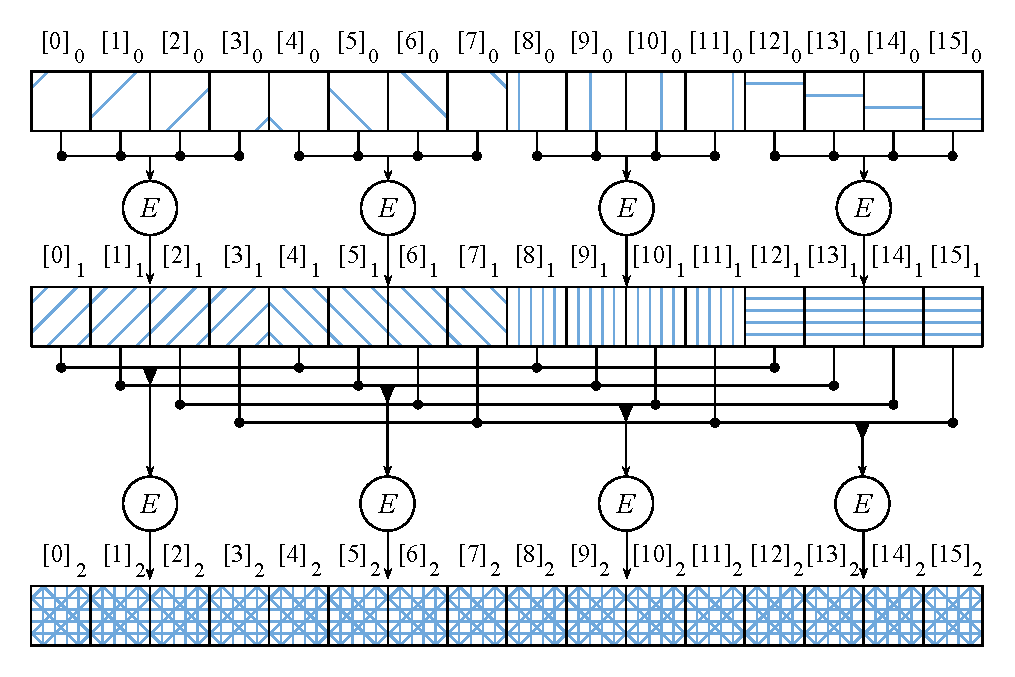
\includegraphics[width=0.9\columnwidth]{figures/fig01}
\caption{\label{ms:fig:mixing} An example of mixing of 16 mini-blocks assuming $m=4$}
\end{figure}

\subsection{Mixing}
\label{ms:sect:mixing}

The basic step of our approach (on which we will iteratively build to provide complete mixing within a macro-block) is the application of encryption at the block level. This application is visible at the top of Figure~\ref{ms:fig:mixing}, where the first row reports a sequence of 16 mini-blocks ($[0],\ldots,[15]$) composing 4 blocks. The second row is the result of block encryption on the sequence of mini-blocks. As visible from the pattern-coding in the figure, encryption provides mixing within each block so that each mini-block in the result is dependent on every mini-block in the same input block. In other words, each $[i]_1$ is dependent on every $[j]_0$ with ($i$ \mydiv 4) = ($j$ \mydiv 4).

One round of block encryption provides mixing only at the level of block. With reference to our example, mixing is provided among mini-blocks $[0]_0 \ldots [3]_0$, $[4]_0 \ldots [7]_0$, $[8]_0 \ldots [11]_0$, and $[12]_0 \ldots [15]_0$, respectively.
%
\new{ %
Absence of a mini-block from the result will prevent reconstruction only of the plaintext block including it, while not preventing the reconstruction of all the other blocks. For instance, with reference to our example, absence of $[2]_1$ will prevent reconstruction of the first block (mini-blocks $[0]_0, \ldots, [3]_0$) but will not prevent reconstruction of the other three blocks (mini-blocks $[4]_0, \ldots, [15]_0$). Protection at the block level is clearly not sufficient in our context, where we expect to manage resources of arbitrarily large size and would like to provide the guarantee that the lack of any individual mini-block would imply the impossibility (apart from performing a brute-force attack) of reconstructing any other mini-block of the resource. The concept of macro-block, and its extension of block ciphers to operate across blocks, allows us to provide mixing on an arbitrarily long sequence of bits. %
} % end \new

The idea is to extend mixing to the whole macro-block by the iterative application of block encryption on, at each round, blocks composed of mini-blocks that are representative (i.e., belong to the result) of different encryptions in the previous round. Before giving the general definition of our approach, let us discuss the simple example of two rounds illustrated in Figure~\ref{ms:fig:mixing}, where $[0]_1, \ldots, [15]_1$ are the mini-blocks resulting from the first round. The second round would apply again block encryption, considering different blocks each composed of a representative of a different computation in the first round. To guarantee such a composition, we define the blocks input to the four encryption operations as composed of mini-blocks that are at distance 4 (=\mnumb) in the sequence, which corresponds to say that they resulted from different encryption operations in the previous round. The blocks considered for encryption would then be $\langle [0]_1[4]_1[8]_1[12]_1\rangle,$ $\langle [1]_1[5]_1[9]_1[13]_1\rangle,$$ \langle [2]_1[6]_1[10]_1[14]_1\rangle, $$\langle [3]_1[7]_1[11]_1[15]_1 \rangle.$ The result would be a sequence of 16 mini-blocks, each of which is dependent on each of the 16 original mini-blocks, that is, the result provides mixing among all 16 mini-blocks, as visible from the pattern-coding in the figure. With 16 mini-blocks, two rounds of encryption suffice for guaranteeing mixing among all of them. Providing mixing for larger sequences clearly requires more rounds. This brings us to the general formulation of our approach operating at the level of macro-block of arbitrarily large size (the example just illustrated being a macro-block of 16 mini-blocks).

Absence of a mini-block from the result will prevent reconstruction of the whole plaintext. With reference to our example in Figure~\ref{ms:fig:unmixing}, absence of $[5]_2$ will prevent reconstruction of the block $\langle [1]_1[5]_1[9]_1[13]_1\rangle$, which in turn will prevent reconstruction of the macro-blocks $[0]_0, \ldots, [15]_0$.

\begin{figure}[!t]
	\centering
	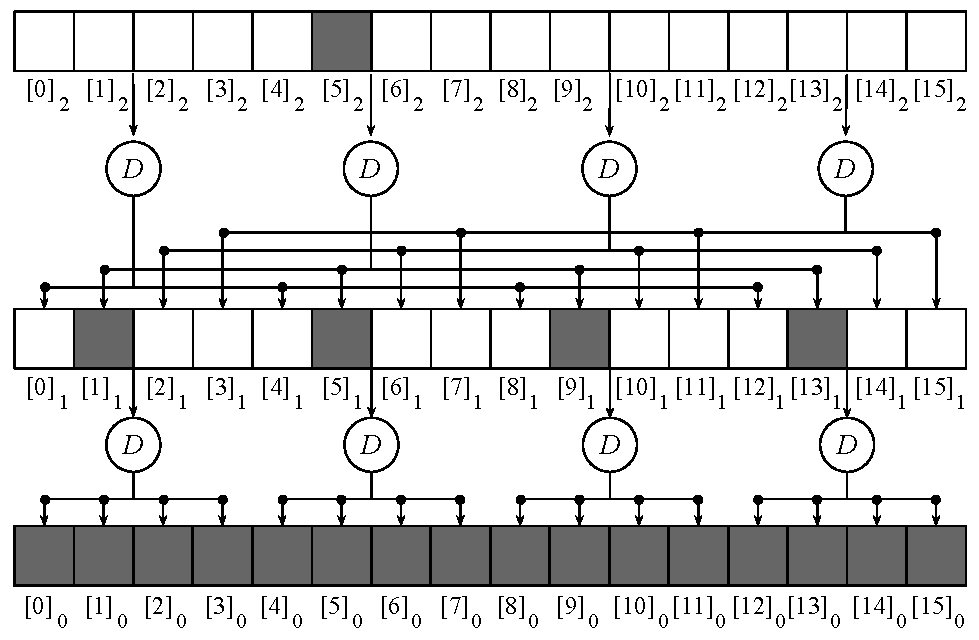
\includegraphics[width=0.9\columnwidth]{figures/decrypt}
	\caption{\label{ms:fig:unmixing} An example of un-mixing of 16 mini-blocks assuming $m=4$}
\end{figure}

To ensure the possibility of mixing, at each round, blocks composed of mini-blocks resulting from different encryption operations of the previous round, we assume a macro-block composed of a number of mini-blocks, which is the power of the number (\mnumb) of mini-blocks in a block. For instance, with reference to our running example where blocks are composed of 4 mini-blocks (i.e., \mnumb=4), macro-blocks can be composed of $4^x$ mini-blocks, with an arbitrary $x$ ($x$=2 in the example of Figure~\ref{ms:fig:mixing}). The assumption can be equivalently stated in terms of blocks, where the number of blocks \bnum\ will be $4^{x-1}$. Any classical padding solution can be employed to guarantee such a requirement, if not already satisfied by the original bit sequence in input.

\begin{figure}[!t]
\begin{small}
\hrule          %
\begin{tabbing}
\hfill\\
{\bf Mix}(\macroblock{})\\[1em]
\num{1:~}\= \myfor\ $i:= 1, \ldots, x$ \com{do} \comm{at each round $i$}\\[0.3em]
\num{2:~}\2 \spanna\ := \mnumb$^i$  \comm{number of mini-blocks in a mixing}\\[0.3em]
\num{3:~}\2 \distance\ := \mnumb$^{i -1}$ \comm{leg of mini-blocks input to an encryption}\\[0.3em]
\num{4:~}\2 \myfor\ $j:= 0, \ldots, \bnum -1$ \com{do} \comm{each $j$ is an encryption}\\[0.3em]
             \3 \comm{identify the input to the $j$-th encryption picking,}\\[0.3em]
             \3 \comm{within each span, mini-blocks at leg \distance}\\[0.3em]
\num{5:~}\3 let \= {\em block} be the concatenation of all mini-blocks $[l]$\\[0.3em]
\num{6:~}\4 s.t.\= \ $(l\mod\distance) = j$ and  \\[0.3em]
\num{7:~}\5 ($j \cdot \mnumb$) \mydiv \spanna\ = $l$ \mydiv \spanna\\[0.3em]
\num{8:~}\3 $[[j]]_i := E(k,block)$ \comm{write the result as the $j$-th block in output}
\end{tabbing}
\hrule
\vspace{.5em}
\end{small}
\caption{\label{ms:fig:encrypt}Mixing within a macro-block \macroblock{}}
\end{figure}

Providing mixing of a macro-block composed of \bnum\ blocks with \bnum=\mnumb$^{x-1}$ requires $x$ rounds of encryption each composed of \bnum\ encryptions. Each round allows mixing among a number \spanna\ of mini-blocks that multiplies by \mnumb\ at every round. At round $i$, each encryption $j$ takes as input \mnumb\ mini-blocks that are within the same \spanna\ (i.e., the same group of $\mnumb^i$ mini-blocks to be mixed) and at a \distance\ ($\mnumb^{i-1}$). Figure~\ref{ms:fig:encrypt} illustrates the mixing procedure. To illustrate, consider the example in Figure~\ref{ms:fig:mixing}, where blocks are composed of 4 mini-blocks (\mnumb=4) and we have a macro-block of 16 mini-blocks, that is, 4 blocks (\bnum=4). Mixing requires $x=2$ rounds of encryption ($16=4^2$), each composed of 4 (\bnum) encryptions operating on 4 (\mnumb) mini-blocks. At round 1, the \spanna\ is 4 (i.e., mixing operates on chunks of 4 mini-blocks) and mini-blocks input to an encryption are taken at distance 1 within each span. At round 2, the \spanna\ is 16 (all mini-blocks are mixed) and mini-blocks input to an encryption are taken at \distance\ 4 within each \spanna. Let us consider, as an another example, a macro-block composed of 64 mini-blocks (i.e., 16 blocks). Mixing requires 3 rounds. The first two rounds would work as before, with the second round producing mixing within chunks of 16 mini-blocks. The third round would then consider a \spanna\ of all the 64 mini-blocks and mini-blocks input to an encryption would be the ones at \distance\ 16.

At each round $i$, mini-blocks are mixed among chunks of $\mnumb^i$ mini-blocks, hence ensuring at round $x$, mixing of the whole macro-block composed of $\mnumb^x$ mini-blocks.

\begin{figure*}[!t]
	\centering
	{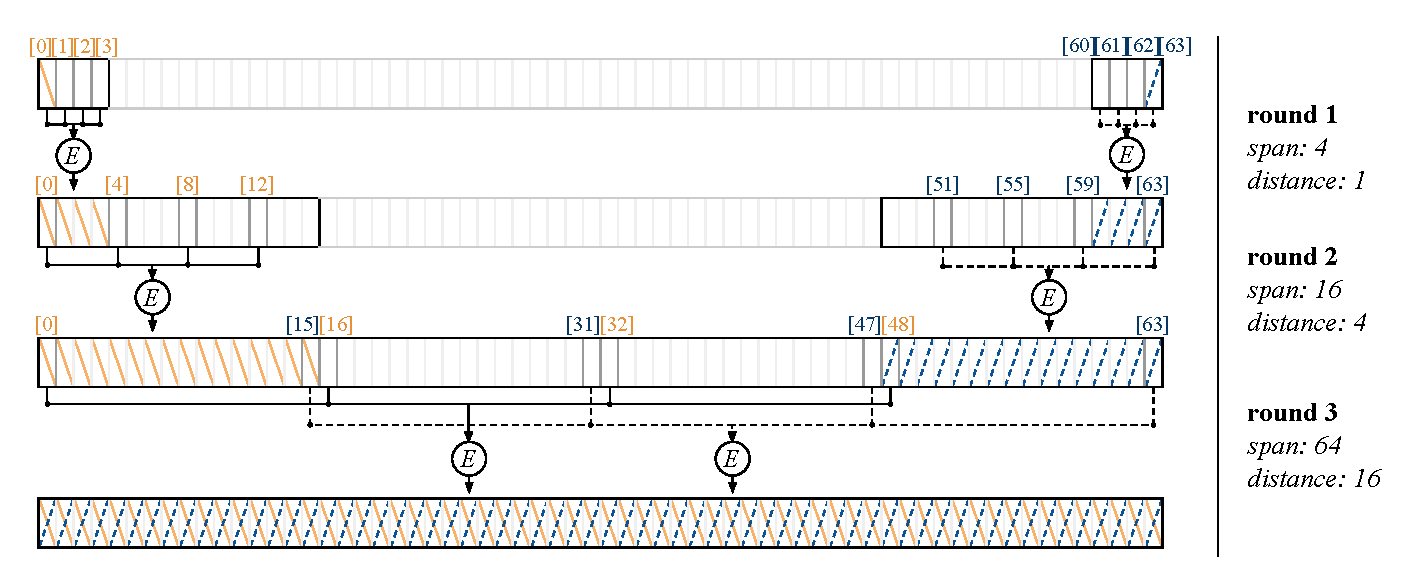
\includegraphics[width=\columnwidth]{figures/fig03}}
	\caption{\label{ms:fig:general}Propagation of the content of mini-blocks [0] and [63] in the mix process}
\end{figure*}

Figure~\ref{ms:fig:general} captures this concept by showing the mixing of the content of the first ([0]) and last ([63]) mini-blocks of the macro-block at the different rounds, given by the encryption to which they (and those mini-blocks mixed with them in previous rounds) are input, showing also how the two meet at the step that completes the mixing. While for simplicity the figure pictures only propagation of the content of two mini-blocks, note that at any step they (just like other mini-blocks) actually carry along the content of all the mini-blocks with which they mixed in previous rounds. Given a macro-block \macroblock{} with \mnumb$^x$ mini-blocks (corresponding to \bnum\ blocks), the following two properties hold: {\em 1)\/} a generic pair of mini-blocks $[i]$ and $[j]$ mix at round $r$ with $i$ \mydiv\ \mnumb$^r$ = $j$ \mydiv\ \mnumb$^r$; and {\em 2)\/} $x$ rounds bring complete mixing. In other words, the number of encryption rounds needed to mix a macro-block with $\mnumb \cdot \bnum$ mini-blocks is $\log_{\mnumb}(\mnumb\cdot\bnum)$.

An important feature of the mixing is that the number of bits that are passed from each block in a round to each block in the next round is equal to the size of the mini-block. This guarantees that the uncertainty introduced by the absence of a mini-block at the first round ($2^{\msize}$) maps to the same level of uncertainty for each of the blocks involved in the second round, and iteratively to the next rounds, thanks to the use of AES at each iteration. This implies that a complete mixing of the macro-block requires at least  $\log_{\mnumb} (\mnumb \cdot \bnum)$ rounds, that is, the rounds requested by  our technique.

Another crucial aspect is that the representation after each round has to be of the same size as the original macro-block. In fact, if the transformation produced a more compact representation, there would be a possibility for a user to store this compact representation and maintain access to the resource even after revocation (this is a weakness of other solutions discussed in Section~\ref{ms:sec:relwork}). Since, in our approach, each round produces a representation that has the same macro-block size, the user has no benefit in aiming to attack one round compared to another (see Section~\ref{ms:sec:security}).

We note that an interpretation of the proposed mixing is that it extends the ability of protecting the correspondence between input and output of a block cipher to blocks of arbitrary size. An alternative approach that we considered to obtain this result was based on the use of a Feistel architecture~\cite{lr88}, which is known to be an effective technique for the construction of block ciphers. The approach uses, as the {\em round} function of the Feistel architecture, a block cipher. The approach can be applied iteratively, doubling the block size at every iteration. The analysis we performed showed that this approach would lead to less efficiency compared to the solution proposed in this chapter, with a number of invocations of the basic block cipher equal to $2\cdot \log_{\mnumb} (\mnumb \cdot \bnum)$. The Feistel-based approach can be adopted when the mini-block size desired for security goes beyond the block size of the available block cipher. Similarly, symmetric cryptosystems operating on large blocks can support larger mini-blocks and also reduce the number of rounds of our approach. For instance, AESQ~\cite{paeq,paeq2} shuffles 4 AES blocks and could be used as a 512-block cipher in our structure.

\new{

\subsection{OAEP mixing}
\label{ms:sect:oaep}

\begin{figure*}[!t]
	\centering
	{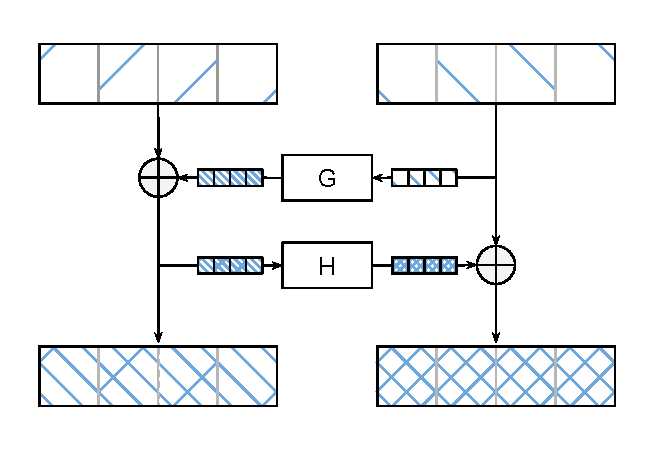
\includegraphics[width=.6\columnwidth]{figures/oaep-issue}}
	\caption{Classical OAEP does not evenly mix the plaintext}
	\label{ms:fig:oaep-issue}
\end{figure*}

Another approach that provides strong inter-dependency in the representation of a resource is {\em Optimal Asymmetric Encryption Padding} (OAEP) \cite{bellare1995optimal, bellare1998relations} proposed by Bellare and Rogaway. OAEP is a Feistel network \cite{feistel1973cryptography} that uses a pair of cryptographically one-way trapdoor functions, $G$ and $H$, to process the plaintext prior to asymmetric encryption. The OAEP process is represented in Figure~\ref{ms:fig:oaep-issue}.
Boyko proved that OAEP can be used to build an All-or-Nothing Transform that is resistant to chosen-plaintext attacks \cite{Boy99}. However, the classical OAEP schema does not imply an {\em Avalanche Effect} \cite{webster1985design}: the change of one bit in the left half of the plaintext, impacts the whole right half, but only affects the corresponding bit in the left half, as shown in Figure~\ref{ms:fig:oaep-issue}. Luby and Rackoff showed in \cite{lr88} that an adaptation of OAEP composed of three rounds instead of two, guarantees that the change of any bit in the plaintext has the chance of affecting any bit in the ciphertext.

Another limitation of the use of OAEP as an AONT is that by construction the output size is $|G_{out}| + |H_{out}|$.
A trivial technique that can be adopted to extend the output of the functions to fit plaintext of any size is to use $G_{out}$ and $H_{out}$ to seed stream ciphers (e.g., RC4), that produce the required number of bits needed for the exclusive-or operation.
Even if efficient, this schema would not be as strong as the original \name. In fact the two seeds $G_{out}$ and $H_{out}$, which are compact in size, can be stored by the adversary to trivially invert the schema even when part of the ciphertext is missing, thus breaking the All-or-Nothing transform.

To solve this problem, we can leverage the Mixing algorithm detailed in Section~\ref{ms:sect:mixing} and replace the encryption function with OAEP.
We can use $G = H = SHA2$ and impose $|G_{in}| = |G_{out}|$ and $|H_{in}| = |H_{out}|$, so that by using $SHA2_{256}$ we can achieve $\msize = 256\ bits$ and $\bsize = 512\ bits$ (each round mixes two mini-blocks). If we need even more protection we can use $SHA2_{512}$ and obtain $\msize = 512\ bits$ and $\bsize = 1024\ bits$. OAEP does not provide message secrecy, so it is required to encrypt the output of the process. In our implementation, we used {\em AES} in {\em CTR mode} to encrypt the output of the OAEP process.

As it will be described in details in Section~\ref{ms:sect:experiments}, the use of AES is computationally efficient due to its hardware implementation available in most of the modern CPUs, however the maximum mini-block size is capped to 64 bits. On the other hand, OAEP with SHA2 does not benefit from hardware implementation, thus it has a lower throughput, yet it enables mini-blocks to be as big as 512 bits, thus enabling the use of \name in scenario that require higher protection from brute-force attacks.

} % end \new


\begin{comment}
To solve this problem, we need to impose constraints over $G$ and $H$.
\vspace{1ex}

\begin{description}
\item [{\em Req.1}] \hspace{1ex} $G$ ($H$) must not have an internal state that can be efficiently stored to reproduce $G_{out}$ ($H_{out}$, respectively).
\item [{\em Req.2}] \hspace{1ex} Any bit changed in $G_{in}$ ($H_{in}$) must have the chance of cryptographically affect (with a uniform distribution of probability) any bit of $G_{out}$ ($H_{out}$, respectively).
\item [{\em Req.3}] \hspace{1ex} $|G_{in}| = |G_{out}|$ and $|H_{in}| = |H_{out}|$, so that an adversary does not have an advantage in storing the input or the output.
\end{description}
\vspace{1ex}

\name complies with all of these requirements and can thus be {\em Req.1} and {\em Req.2} imply that $G$ and $H$ has to be whitebox-AONTs. The mixing technique presented in Section~\ref{ms:sect:mixing} is a whitebox-AONT and also satisfies {\em Req.3}, therefore it can be used as $G$ and $H$.

Moreover, since in the OAEP schema, $G$ and $H$ do not need to be invertible, we can replace the use of AES with the use of {\em sha-512} in the mixing process. This way, with the size of the mini-block being equal, the use of {\em sha-512}, which has a \bsize\ of 512 bits, permits to exponentially reduce the number of rounds in the mixing process, since it is now possible to mix $16$ mini-blocks in one step (with \msize\ $= 32$).
Another advantage of the use of {\em sha-512} is that the mini-block size can increase up to $256$ bits, for applications that require a stronger protection from brute-force attacks.


%The overall schema is presented in Figure~\ref{ms:fig:oaep}.
In section~\ref{ms:sect:experiments} we compare the two proposed implementations.
\end{comment}

\subsection{Shortcomings of large macro-blocks}

When resources are extremely large (or when access to a resource involves only a portion of it) considering a whole resource as a single macro-block may be not desirable. Even if only with a logarithmic dependence, the larger the macro-block the more the encryption (and therefore decryption to retrieve the plaintext) rounds required. Also, encrypting the whole resource as a single macro-block implies its complete download at every access, when this might actually not be needed for service.

Accounting for this, we do not assume a resource to correspond to an individual macro-block, but assume instead that any resource can be partitioned into \Mnum\ macro-blocks, which can then be mixed independently. The choice of the size of macro-blocks should take into consideration the performance requirements of both the data owner (for encryption) and of clients (for decryption), and the possible need to serve fine-grained retrieval of content. This requirement can be then efficiently accommodated independently encrypting (i.e., mixing) different portions of the resource, which can be downloaded and processed independently (we will discuss this in Section~\ref{ms:sec:overlay}).

Encryption of a resource would then entail a preliminary step cutting the resource in different, equally sized, macro-blocks on which mixing operates. To ensure the mixed versions of macro-blocks be all different, even if with the same original content, the first block of every macro-block is {\sc xor}ed with an {\em initialization vector\/} (\var{IV}) before starting the mixing process. Since mixing guarantees that every block in a macro-block influences every other block, the adoption of a different initialization vector for each macro-block guarantees indistinguishability among their encrypted content. The different initialization vectors for the different blocks can be obtained by randomly generating a vector for the first macro-block and then incrementing it by 1 for each of the subsequent macro-blocks in the resource, in a way similar to the CTR mode~\cite{d01}. Figure~\ref{ms:fig:mixslice}(a) illustrates such process.

\begin{figure}[!t]
\centering
{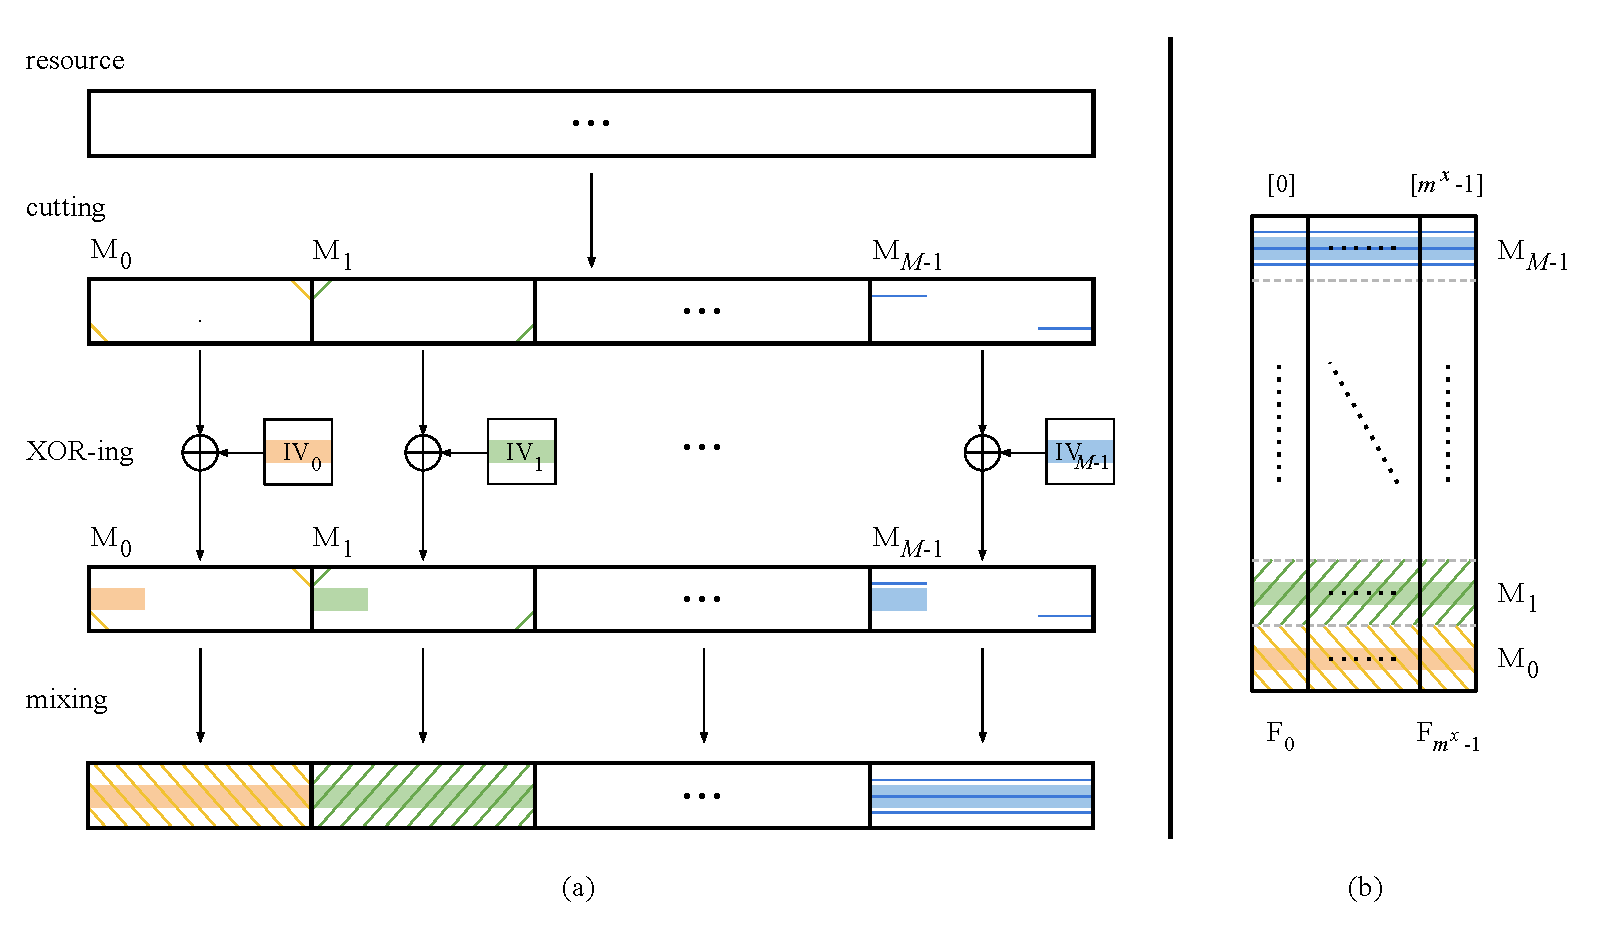
\includegraphics[width=\columnwidth]{figures/fig04}}
\caption{\label{ms:fig:mixslice} From resource to fragments}
\end{figure}

\subsection{Slicing}

The starting point for introducing mixing is to ensure that each single bit in the encrypted version of a macro-block depends on every other bit of its plaintext representation, and therefore that removing any one of the bits of the encrypted macro-block would make it impossible (apart from brute-force attacks) to reconstruct any portion of the plaintext macro-block. Such a property operates at the level of macro-block. Hence, if a resource (because of size or need of efficient fine-grained access) has been partitioned into different macro-blocks, removal of a mini-block would only guarantee protection of the macro-block to which it belongs, while not preventing reconstruction of the other macro-blocks (and therefore partial reconstructions of the resource). Resource protection can be achieved if, for each macro-block of which the resource is composed, a mini-block is removed. This observation brings to the second concept giving the name to our approach, which is {\em slicing}. Slicing the encrypted resource consists in defining different {\em fragments} such that a fragment contains a mini-block for each macro-block of the resource, no two fragments contain the same mini-block, and for every mini-block there is a fragment that contains it. To ensure all this, as well as to simplify management, we slice the resource simply putting in the same fragment the mini-blocks that occur at the same position in the different macro-blocks. Slicing and fragments are defined as follows.

\begin{dfn}[Slicing and fragments]
\sloppy{
Let \resource\ be a resource and $\macroblock{0},\ldots,\macroblock{\Mnum-1}$ be its (individually mixed) macro-blocks, each composed of $(\mnumb \cdot \bnum)$ mini-blocks. Slicing produces $(\mnumb \cdot \bnum)$ fragments for \resource\ where $\fragment{\var{i}}{}=\langle\miniinmacro{0}{\var{i}},\ldots,\miniinmacro{\Mnum-1}{\var{i}}\rangle$, with $i=1,\ldots,(\mnumb \cdot \bnum)$.
}
\end{dfn}

Figure~\ref{ms:fig:mixslice}(b) illustrates the slicing process and Figure~\ref{ms:fig:algoenc} illustrates the procedure for encrypting a resource \resource. \resource\ is first cut into \Mnum\ macro-blocks and an initialization vector is randomly chosen. The first block of each macro-block is then {\sc xor}-ed with the initialization vector, which is incremented by 1 for each macro-block. The macro-block is then encrypted with a mixing process (Figure~\ref{ms:fig:encrypt}). Encrypted macro-blocks are finally sliced into fragments.
